\section{实验}
\subsection{协议}
主模型为 Meta-Llama-3.1-8B-Instruct。共同 Vector-GSQ 锚点量化 32 层、224 个 Linear；FineWeb-Edu 使用 4096/128 条 4096-token 文本，Vector-GPTQ 使用 512 条。适应只开放 layers 28--31，任务训练/验证各为每任务 512/256 条，文本为 4096/128 条，训练 2 epochs。Joint final audit 使用未被前序实验读取的每任务 64 条和新 C4 64 条。PPL 使用 WikiText2 raw test、seqlength 2048；准确率使用 \texttt{lm\_eval 0.4.4} 全量 0-shot ARC-C、ARC-E、HellaSwag、LAMBADA、PIQA、WinoGrande。所有正式实验仅暴露一张 A100 80GB，不扫描 seed、group size 或学习率。

\begin{figure*}[t]
  \centering
  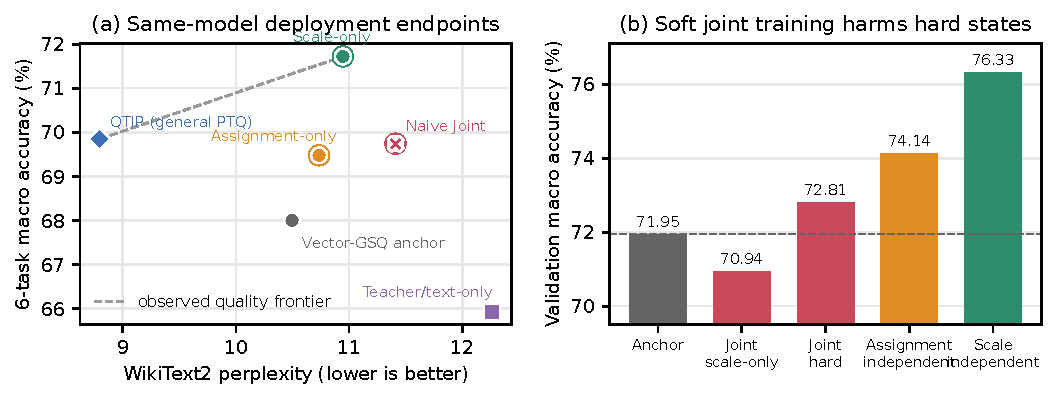
\includegraphics[width=\textwidth]{../img/v9_coordinate_pareto.pdf}
  \caption{左：同模型部署端点的 WikiText2 PPL--Macro-6；外圈点使用目标任务监督。右：joint 中只保留尺度的零切换硬状态低于锚点，入选 hard joint 仍低于两个独立坐标。}
  \label{fig:pareto-hard-state}
\end{figure*}

\subsection{主要结果}
\begin{table}[t]
\centering
\small
\caption{同一锚点上的完整部署结果。最佳任务分数加粗。}
\begin{tabular}{lrrr}
\toprule
端点 & PPL$\downarrow$ & Macro-6$\uparrow$ & 五任务$\uparrow$\\
\midrule
Vector-GSQ anchor & \textbf{10.4960} & 67.9997 & 68.1046\\
Teacher/text-only & 12.2604 & 65.9217 & 67.2062\\
Task-assignment & 10.7347 & 69.4774 & 69.0744\\
Task-scale & 10.9448 & \textbf{71.7223} & \textbf{72.5484}\\
Naive joint & 11.4098 & 69.7434 & 68.9511\\
\bottomrule
\end{tabular}
\label{tab:main}
\end{table}

尺度相对锚点提高 3.7225/4.4438 pp Macro-6/五任务，PPL 退化 4.2757\%；assignment 提高 1.4777/0.9698 pp，PPL 退化 2.2742\%。两者因而是不同 task--PPL 端点。Joint 选择 epoch 1 的 1/2 投影，改变 0.860971\% assignment；全部 5,521,408 个尺度 delta 非零。它在全新 audit 上使 balanced loss 降低 8.5607\%、文本 CE 降低 1.9967\%，但正式 Macro-6/五任务比 scale-only 低 1.9789/3.5972 pp，PPL 高 4.2489\%。Scale-only 在三个指标上严格支配 joint。

\subsection{Hard-state 诊断}
Joint epoch 1 的零切换尺度端点验证 Macro 为 70.9375\%，低于锚点 71.9531\%；入选 hard joint 为 72.8125\%，仍低于独立 assignment 的 74.1406\% 和独立尺度的 76.3281\%。若失败仅源于保留过多 switch，零切换应接近独立尺度；反例说明尺度已经补偿 soft codeword mixture，hard projection 后无法独立部署。

独立 assignment 也显示 hard trust region：1/8、1/4、1/2、full 投影的切换率为 0.3781\%、0.7562\%、1.5124\%、3.0248\%，验证准确率依次为 74.1406\%、73.6719\%、73.4375\%、71.5625\%。附近领域限制单步半径，但不能保证大量离散步组合后仍有收益。

\subsection{外部边界与代价}
同模型 QTIP 统一复现为 2.00 bpp、PPL 8.7971、五任务 69.8749\%；公开 GSQ 质量点为 2.13 bpp、五任务 68.55\%。任务尺度的平均数值更高，但使用目标任务 training split 且 PPL 更差，不能据此声称通用 PTQ SOTA。PV-Tuning 已提供更一般的连续--离散坐标优化框架；本文只主张特定部署失配证据。

完整锚点量化约 54.58 小时；尺度、assignment 与 joint 适应分别为 1.49、6.45 与 7.56 小时。Joint 峰值显存 35.16 GiB。三者不增加逻辑 bpp，且 checkpoint 的固定字段、fresh reconstruction 与 dtype 审计通过。当前证据只覆盖一个 8B Instruct 模型、固定 seed 和最后四层；没有定制推理 kernel，也尚未运行 hard-checkpoint 分阶段修复。
